\chapter{Pourquoi ce dossier?}

Ce dossier fait le bilan des premières années d'expérimentations qui se sont écoulées dans votre ferme et dans le réseau de fermes.
Il permet de vous accompagner dans votre sélection d'un point de vue agronomique.
Il n'est pas question ici de la qualité du blé, de son comportement en panification.
Cet aspect qualité sera intégré dans le futur.

\warning{Ce dossier n'est qu'un modeste complément de l'expertise que vous avez développé en observant les populations chez vous, dans les champs et peut être au fournil.}

Ce document est séparé en deux parties:

\begin{enumerate}

\item \textbf{Une première partie traite des résultats dans votre ferme.} Cette partie permet de vous orienter pour répondre à la question : \textbf{Quelles populations se comportent le mieux dans ma ferme?}

Pour cela nous vous donnons les données recueillies pour chaque étape du cycle de la population (automne, hiver, printemps et été) ainsi que les mesures qui ont été effectuées au Moulon pour le poids de mille grains, le taux de protéine, le poids des épis, et dans les champs pour la hauteur et la verse.

Pour les personnes concernées, nous vous apportons également des résultats sur vos bouquets de sélection, sur la réponse de ces bouquets à la sélection ainsi que sur l'essai mélange.

\item \textbf{Une deuxième partie traite des résultats dans le réseau de fermes.} Cette partie permet de vous orienter pour répondre à la question : \textbf{Quelles populations serait-il plus intéressant de tester chez moi pour les prochains semis?} Ces résultats vous permettent de mobiliser la diversité évaluée dans le réseau de fermes.

\begin{itemize}
\item Dans un premier temps, nous montrons les fermes dans lesquelles les populations se comportent le plus comme dans  votre ferme. Cela vous permet de vous mettre en lien avec cette ferme afin de récupérer quelques populations.

\item Dans un deuxième temps 

\item Ensuite, nous vous donnons les caractéristiques génétiques des populations, c'est à dire:
\begin{itemize}
\item Leurs effets génétiques (intrinsèque aux populations)
\item Leurs sensibilité à l'interaction. Moins elles sont sensibles à l'interaction, plus elles se comportent moyennement de la même manière dans les fermes par rapport aux autres populations.
\end{itemize}

\item Enfin, nous vous proposons de prédire les valeurs qu'auraient eu certaines populations dans vos fermes cette année : on prédit le passé!
Cette information est issue des modèles statistiques que nous avons développés.
Comme tous modèles, il donne une information avec une certaine confiance qui est donnée en pourcentage.
\end{itemize}

\end{enumerate}

Les graphiques et les tableaux sont expliqués au fur et à mesure du document.
En cas de soucis de compréhension, n'hésitez pas à nous contacter (\href{mailto:pierre@semencespaysannes.org}{pierre@semencespaysannes.org}, 06 87 13 46 98). 
Quand nous n'avons pas eu les données, il n'y a pas de résultats et la mention "Pas de données" apparaît.\\

Au delà de cette diversité disponible dans votre ferme et dans le réseau, vous pouvez développer de nouvelles populations.
Pour cela deux solutions sont à votre disposition\footnote{Il en existe d'autres mais elles sont plus compliquées à mettre en oeuvre. On revient sur ce point lors des formations.} : 

\begin{itemize}
\item mélanger des populations existantes
\item faire des croisements. Dans ce cas, vous pouvez nous envoyer les parents que vous souhaitez croiser. L'équipe de recherche peut les croiser au Moulon. Elle pourra également venir faire des formations afin que vous puissiez réaliser vous même vos croisements dans votre ferme.
\end{itemize}

~\\  

Selon vos souhaits et le nombre de populations que vous voulez semer, nous vous proposerons d'être ferme régionale ou ferme satellite.
La figure ci-dessous rappelle la particularité de ces deux types de fermes.
Avec les témoins : \colorbox{black}{\textcolor{white}{Rouge-du-Roc}}; \colorbox{black}{\textcolor{white}{C14}}; \colorbox{black}{\textcolor{white}{C21}}; \colorbox{black}{\textcolor{white}{Renan}}.
Nous pouvons avoir les plans suivant (ces plans sont modulables selon vos contraintes ...):

\begin{center}
	\begin{tabular}{c c}
	
	Fermes régionales & Fermes satellites \\
	\hline	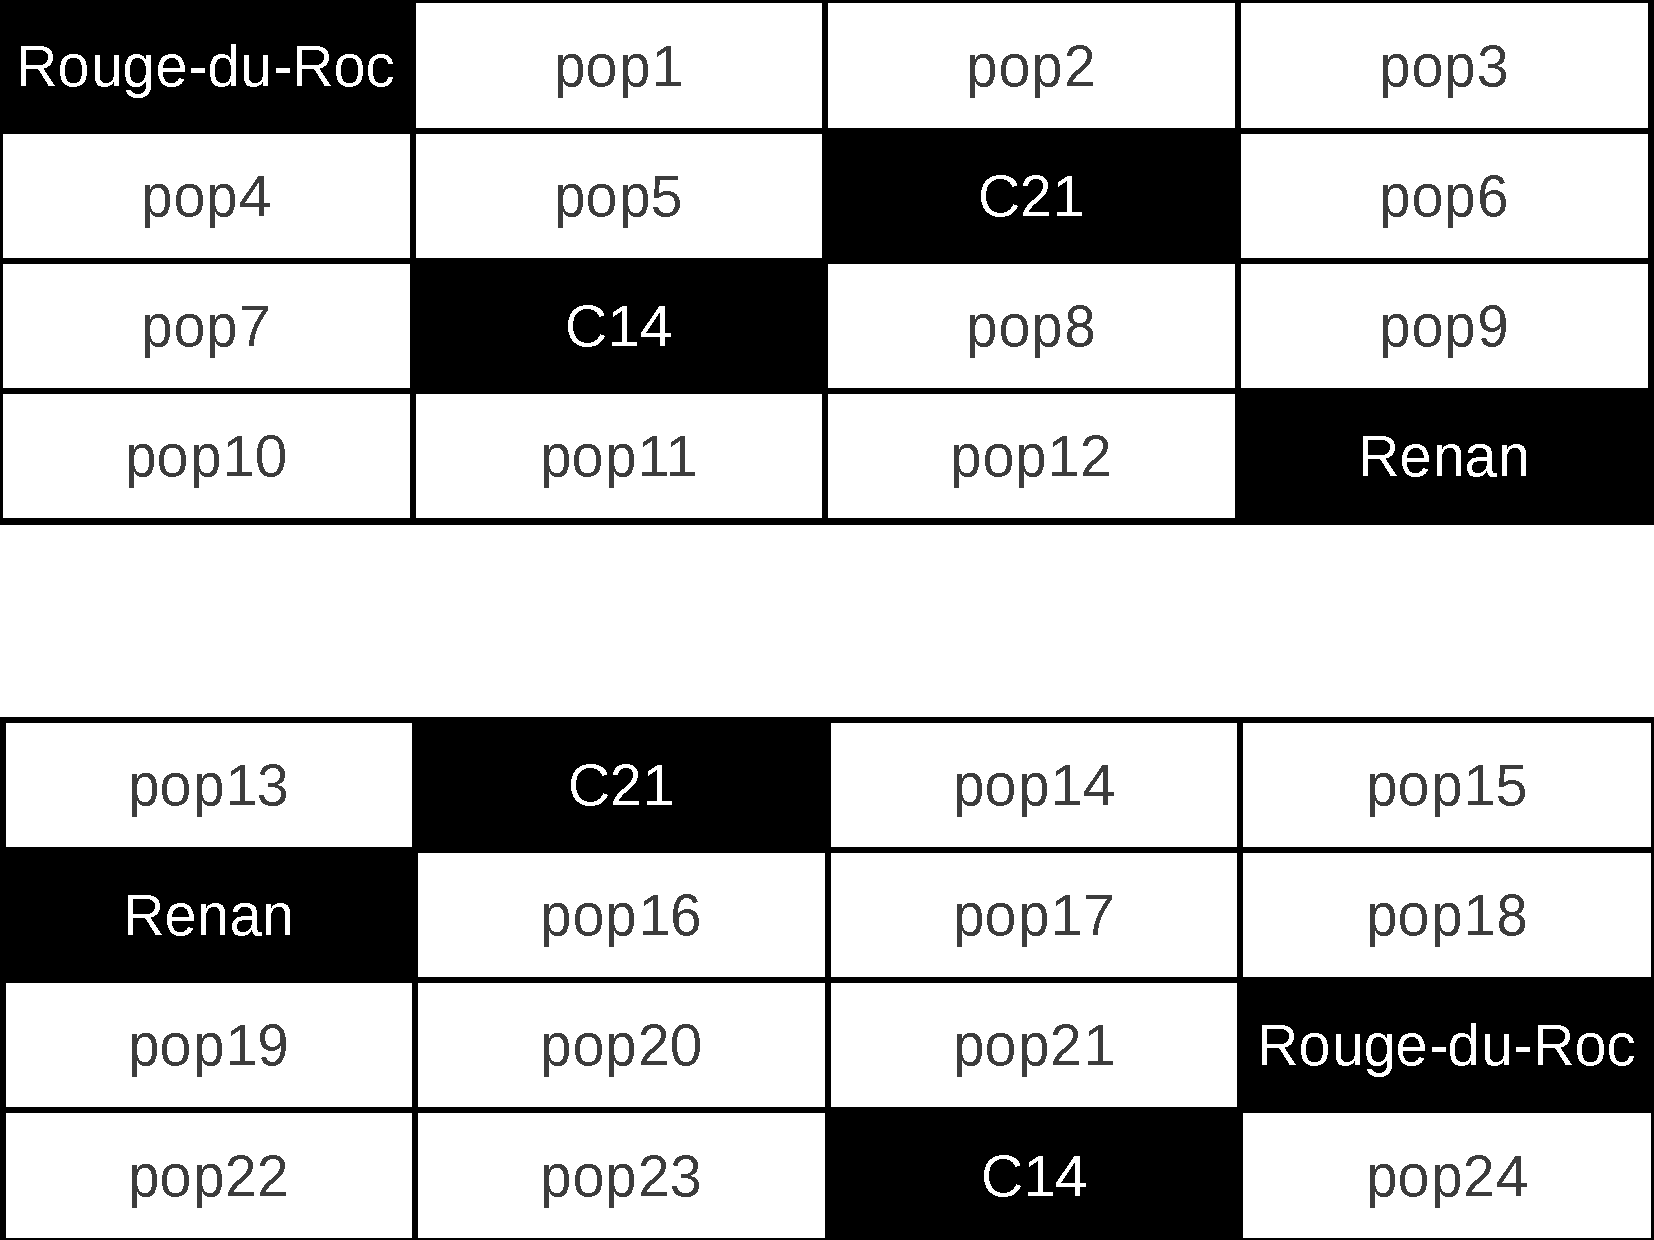
\includegraphics[width=.4\textwidth]{tex_files/plan_FR.pdf} & 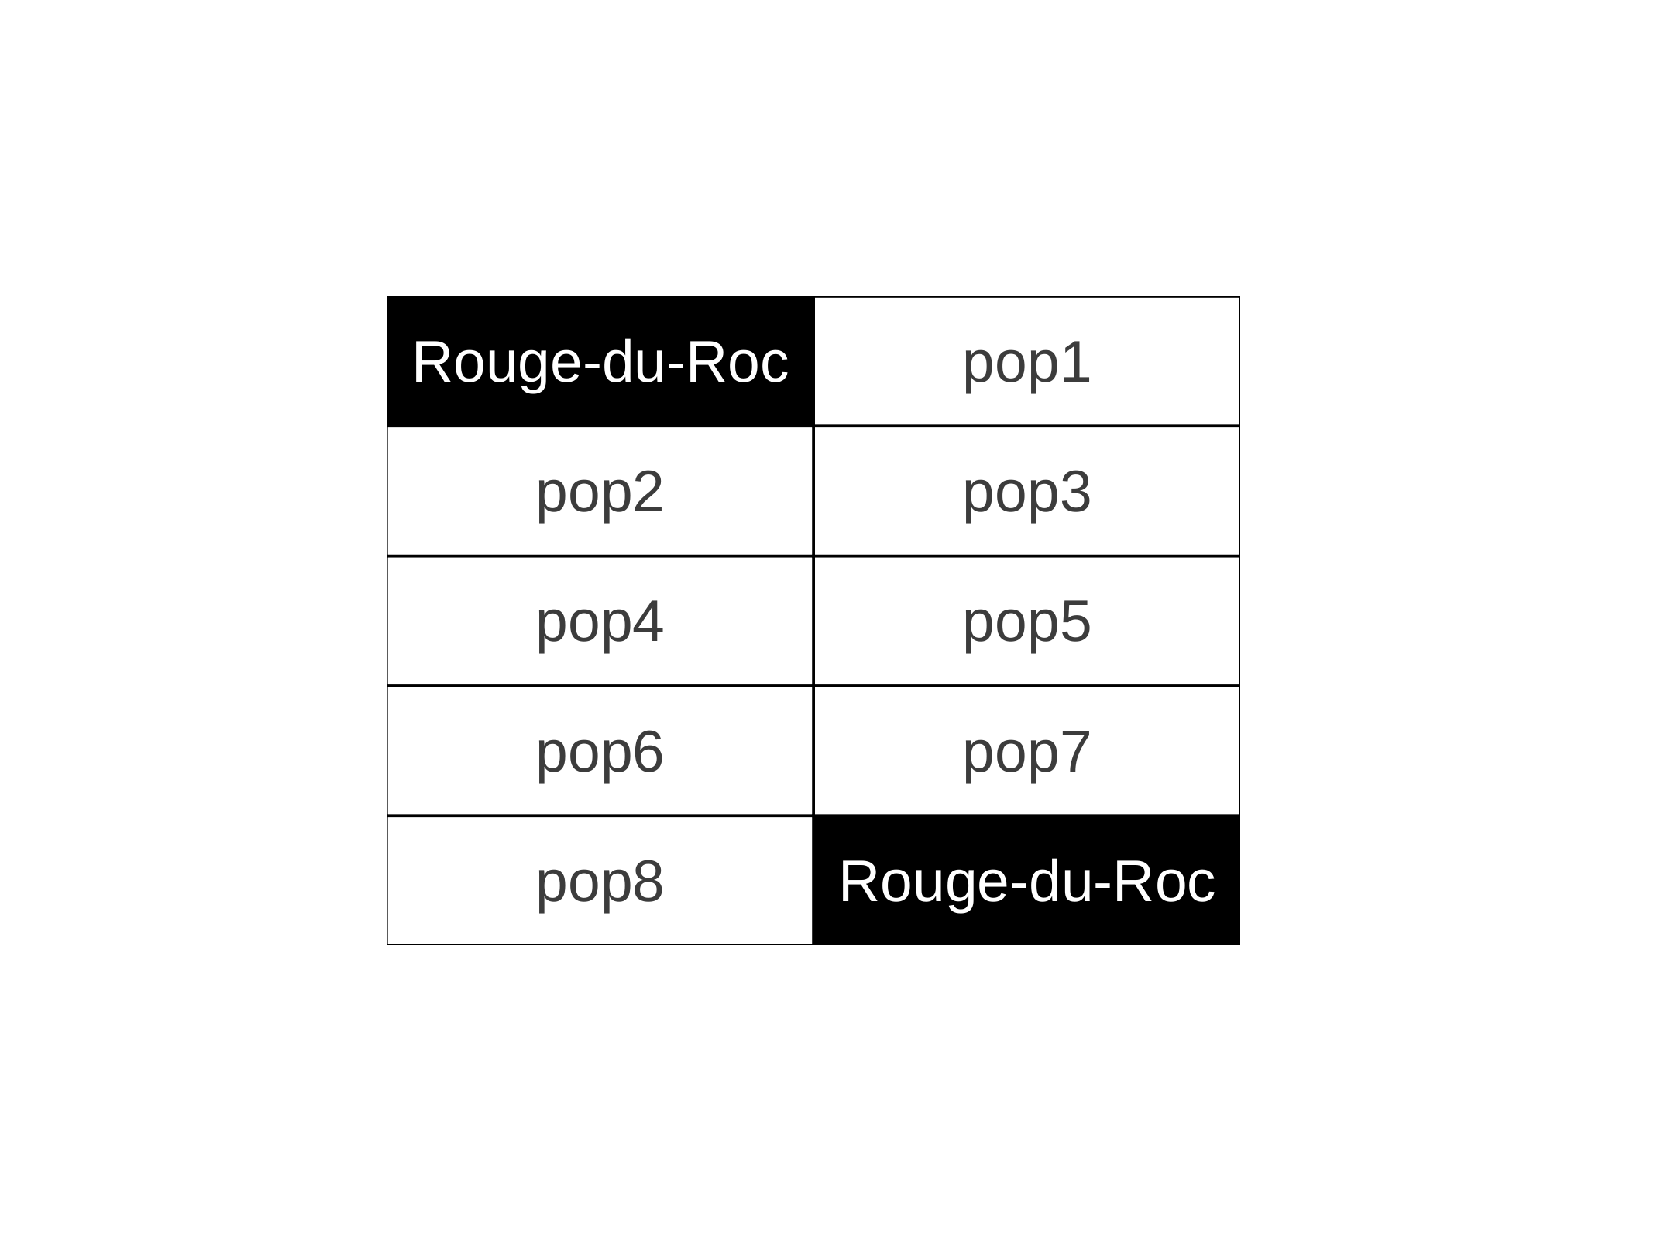
\includegraphics[width=.4\textwidth]{tex_files/plan_FS_bis.pdf} \\
	
	4 témoins dans 2 blocs & pas de blocs; 1 témoin répété deux fois \\

	24 populations non répétées & 8 populations non répétées \\
	\hline
	\end{tabular}
\end{center}

~\\ 

Nous avons joint à ce dossier trois fiches à remplir afin d'avoir 
\begin{itemize}
\item votre avis sur ce dossier. En effet, ce type de retour est en construction et nous avons besoin de vous pour l'améliorer.
%\item la liste des populations que vous souhaitez semer pour les prochains semis. Cela nous permettra de faciliter les échanges de semences et de vous proposer un plan
\item la liste éventuelle de parents que vous souhaiteriez croiser
\end{itemize}


La fiche \guill{Le rôle des paysans participant au projet de sélection collaborative sur les céréales} qui réapitule les différentes étapes du projet est présenté dans la partie 2 de ce document.

\vfill

\begin{flushright}
Bonne lecture et bons semis!

Le Réseau Semences Paysannes

L'équipe DEAP de l'INRA du Moulon
\end{flushright}
\vfill


\newpage

